\section{Design}\label{design}



\subsection{Interface}


Developers using \sys{} write function handlers and define triggers just like
they would for any existing serverless offering. In addition, they asign each
function to a price class, this is done at function creation. For instance, a
simple web server might consist of a home page view that is assigned a higher
priority and costs 2$\mu\cent$ per cpu second, a user profile page view which is
assigned a middle-high priority and cost 1.5$\mu\cent$ per cpu second, and
finally an image processing job that can be set to a low priority which costs
only 0.5$\mu\cent$ per cpu second.

Priorities are inherited across call chains: if a high priority job calls a low
priority job, that invocation with run with high priority. This is important in
order to avoid priority inversion.

Developers pay for memory separately, and by use; the price for memory is the
same across all priorities.

To avoid unexpected costs in the case of for example a DOS attack or a bug,
developers also express a monthly budget that they are willing to pay.\ \sys{}
uses this budget as a guideline and throttles invocations or decreases quality
of service in the case that usage is not within reason given the expected
budget, though it does not guarantee that the budget will not be exceeded by
small amounts.



\subsection{\Sys{} Design}

\begin{figure}[t]
    \centering
      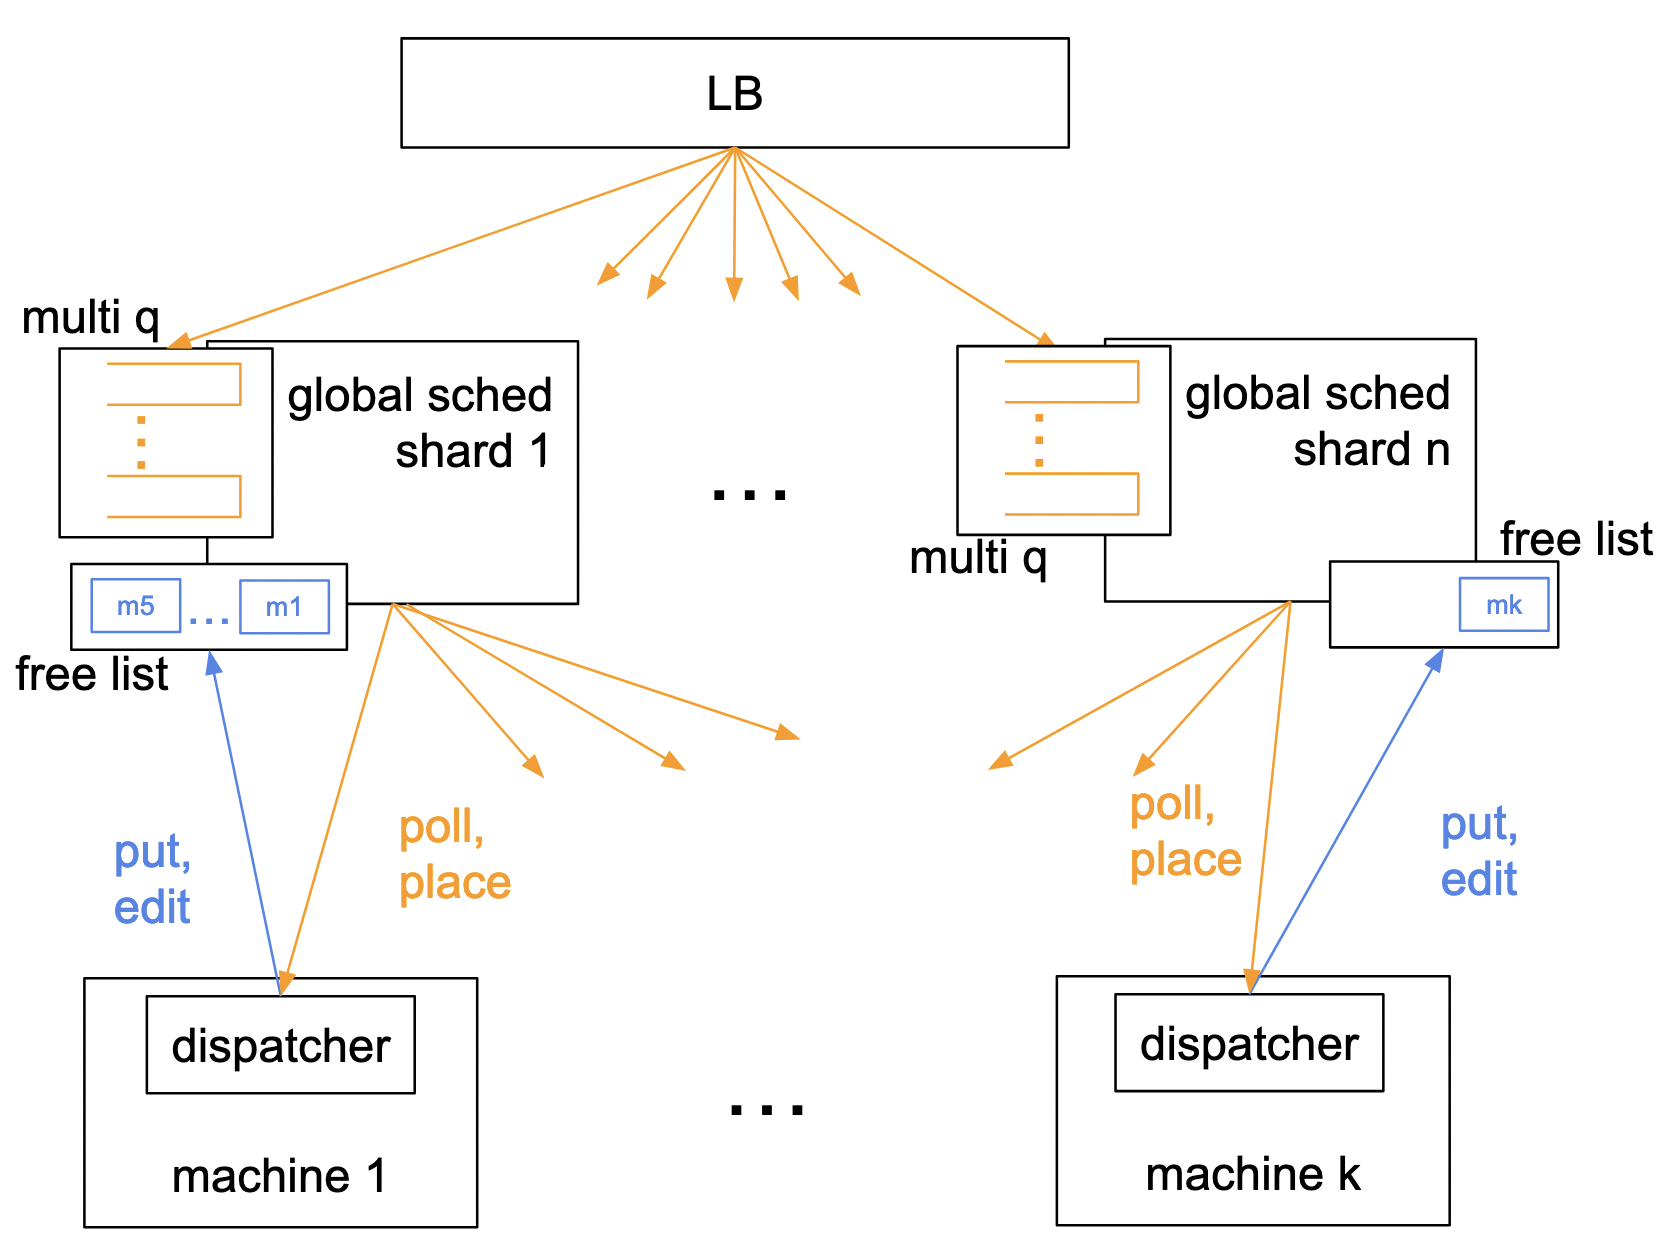
\includegraphics[width=9cm]{img/overview.png}
      \caption{ global scheduler shards queue and place jobs (in orange), 
      on each machine a dispatcher thread keeps track of memory utilization 
      and if it's low writes itself to an idle list (in blue) }
    \label{fig:overview}
\end{figure}



\Sys{} has as its goal to enforce the priorities attached to jobs, which means
it needs to prefer higher priority jobs over lower ones, and preempt the latter
when necessary.
  

As shown in Figure~\ref{fig:overview}, \sys{} sits behind a load balancer, and
consists of: a distributed global scheduler, which places new job invocations, a
dispatcher, which runs on each machine and communicates with the global
scheduler shards, and a machine scheduler, which enforces priorities on the
machines.

Global scheduler shards store the jobs waiting to be placed in a multi queue,
with one queue per priority.

\textbf{Idle list.}
Each global scheduler shard also maintains an \textit{idle list}, which holds
machines that have a significant amount of memory available. In the shards idle
list each machine's entry is associated with the amount of free memory as well
as the current amount of jobs on the machine. The idle list exists because
datacenters are large: polling a small number of machines has been shown to be
very powerful, but cannot find something that is a very rare occurrence.
% join idle queue
What this means is that polling is likely to find a machine in the lower
quantile of the datacenter, but not at the absolute bottom --- it will not find
one of the handful of machines that are actually idle. Having an idle list
allows these machines, which are expected to be rare in a high-utilization
setting, to make themselves visible to the global scheduler. The idle list also
allows the global scheduler to place high priority processes quickly, without
incurring the latency overheads of doing the polling to find available
resources.


\textbf{Machine Scheduler.}
The machine scheduler is a preemptive priority scheduler: it preempts lower
priority jobs to run higher priority ones. Being unfair and starving low
priority jobs is desirable in \sys{}, since image processing jobs should not
interrupt a page view request processing, but vice versa is expected.


\textbf{Dispatcher.}
The dispatcher is in charge of adding itself to a shard's idle list when memory
utilization is low. The dispatcher chooses which list to add itself to using
power-of-k-choices: it looks at k shards' idle lists and chooses the one with
the least other machines in it. If the machine is already on an idle list on
shard $i$, but the amount of available memory has changed significantly (either
by jobs finishing and memory being freed or by memory utilization increasing
because of new jobs or memory antagonists), the dispatcher will update shard
$i$'s idle list. These interactions from the dispatcher to free lists are
represented by the blue arrows in Figure~\ref{fig:overview}.

The dispatcher is most importantly in charge of managing memory. 

\makeatletter
\renewcommand{\ALG@name}{Procedure}
\makeatother
\begin{algorithm}[t]
\caption{Choosing a machine for a job j}\label{alg:place}
\begin{algorithmic}
    \State$N = \{ $ machines in freeList with memAvail > j.maxMem $\}$
    \If{$|N| > 0$} \\
        \Return$ $min(N.maxPriorityRunning, N.qSize)
    \EndIf
    \State$M = $ timeToProfit of k polled machines
    \If{min(M.timeToProfit$) < THRESH$} \\
        \Return$ $min($M$)
    \Else
        \State$ $reQ j, with priority -= 1
    \EndIf
\end{algorithmic}
\end{algorithm}


\textbf{Global Scheduler Shards.}

Shards choose what job to place next by looking at each job at the head of a
queue in the shards multi-queue, and comparing the ratio of priority to amount
of time spent in the queue. This ensures that high priority jobs don't have to
wait as long as lower priority jobs to be chosen next, but low priority jobs
will get placed if they have waited for a while.

When placing the chosen job, the shard finds a machine to run it, shown in
Procedure~\ref{alg:place}. The shard will first look in its idle list for a
machine that has the job's maximum memory available. If there are multiple such
machines, the shard looks at each machines compute pressure metrics; the goal
being to minimize cpu idleness and job latency in low load
settings.\hmng{playing with details of this in the scheduler right now} 

If a machine from the idle list is chosen, the response from the dispatcher upon
placing the job will include updated utilization information, which the shard
will use to update the idle list entry.

If there are no machines in the idle list with the memory available, the shard
switches over to power-of-k-choices: it polls k machines, sending the price and
the maximum memory of the job currently being placed, and getting back the time
to profit. The shard then can choose to place the new job on the machine with
the minimum value, or if all of them are too high the shard re-queues the job.
